\section{Examen des données, prétraitements et extraction des descripteurs}

\textbf{Question 1: Preprocessing Function}

\begin{figure}[!h]
    \begin{minipage}{.40\linewidth}
        \begin{minted}[frame=lines, framesep=2mm, baselinestretch=1.2, fontsize=\footnotesize, linenos, breaklines=true]{python}
def preprocessing():
    img73, img87 = loadImages()
    plt.subplot(1, 2, 1)
    plt.imshow(img73)
    plt.title('Image 1973')
    plt.subplot(1, 2, 2)
    plt.imshow(img87)
    plt.title('Image 1987')
    plt.show()

    return 0, img73, img87
            \end{minted}   
    \end{minipage}\hfill
    \begin{minipage}{.56\linewidth}
        \begin{center}
            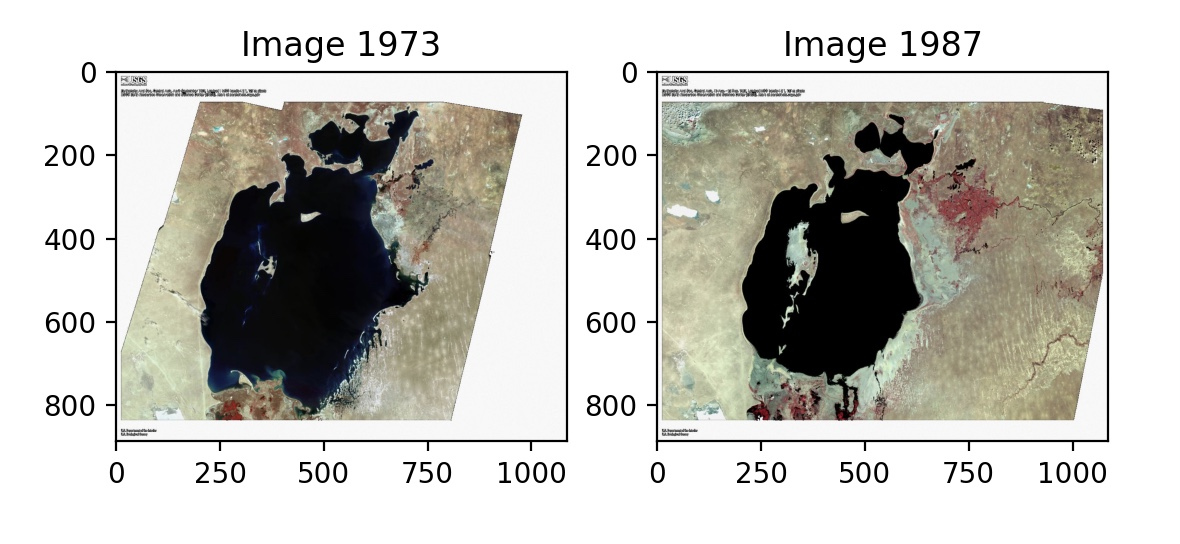
\includegraphics[width=1.0\textwidth]{./img/2.1.jpg}
            \caption{\label{fig:1.2}Images chargées}  
        \end{center}
    \end{minipage}
\end{figure}


\textbf{Question 2: Analyse des images} \\

L'analyse de ces images indique que les dimensions de ces images sont les mêmes. Les valeurs des pixels sont codées sur trois
canaux, en RGB. Au niveau visuel, on distingue nettement la différence de surface entre 1973 et 1987, notamment l'île située 
à l'ouest de la mer d'Aral qui a été multiplié au moins par dix. 

\clearpage

\begin{figure}[!h]
    \begin{minted}[frame=lines, framesep=2mm, baselinestretch=1.2, fontsize=\footnotesize, linenos, breaklines=true]{python}
    featLearn, img73, img87 = preprocessing()
    height, width, channels = img73.shape
    print(f"Image img73 dimensions: Height = {height}, Width = {width}, Channels = {channels}")
    height, width, channels = img87.shape
    print(f"Image img87 dimensions: Height = {height}, Width = {width}, Channels = {channels}")
    """return 
    Image img73 dimensions: Height = 889, Width = 1086, Channels = 3
    Image img87 dimensions: Height = 889, Width = 1086, Channels = 3
    """
    \end{minted}   
    \captionof{listing}{\label{lst:main}Main Function}
\end{figure}

\textbf{Question 3: Dimension de l'espace des descripteurs} \\

L'image étant codée en RGB, cela veut dire que chaque pixel est décrit par trois valeurs qui correspondent à l'intensité du 
Rouge, Vert et Bleu. La dimension de l'espace des descripteurs est donc de trois, on a un espace tridimensionnel. \\

\textbf{Question 4: Images tronquées}

\begin{figure}[!h]
    \begin{minted}[frame=lines, framesep=2mm, baselinestretch=1.2, fontsize=\footnotesize, linenos, breaklines=true]{python}
plt.subplot(1, 2, 1)
plt.imshow(img73)
plt.title('Cropped Image 1973')
plt.subplot(1, 2, 2)
plt.imshow(img87)
plt.title('Cropped Image 1987')
plt.show()
    \end{minted}   
    \captionof{listing}{\label{lst:main}Main Function}
\end{figure}

\begin{figure}[!h]
    \begin{center}
        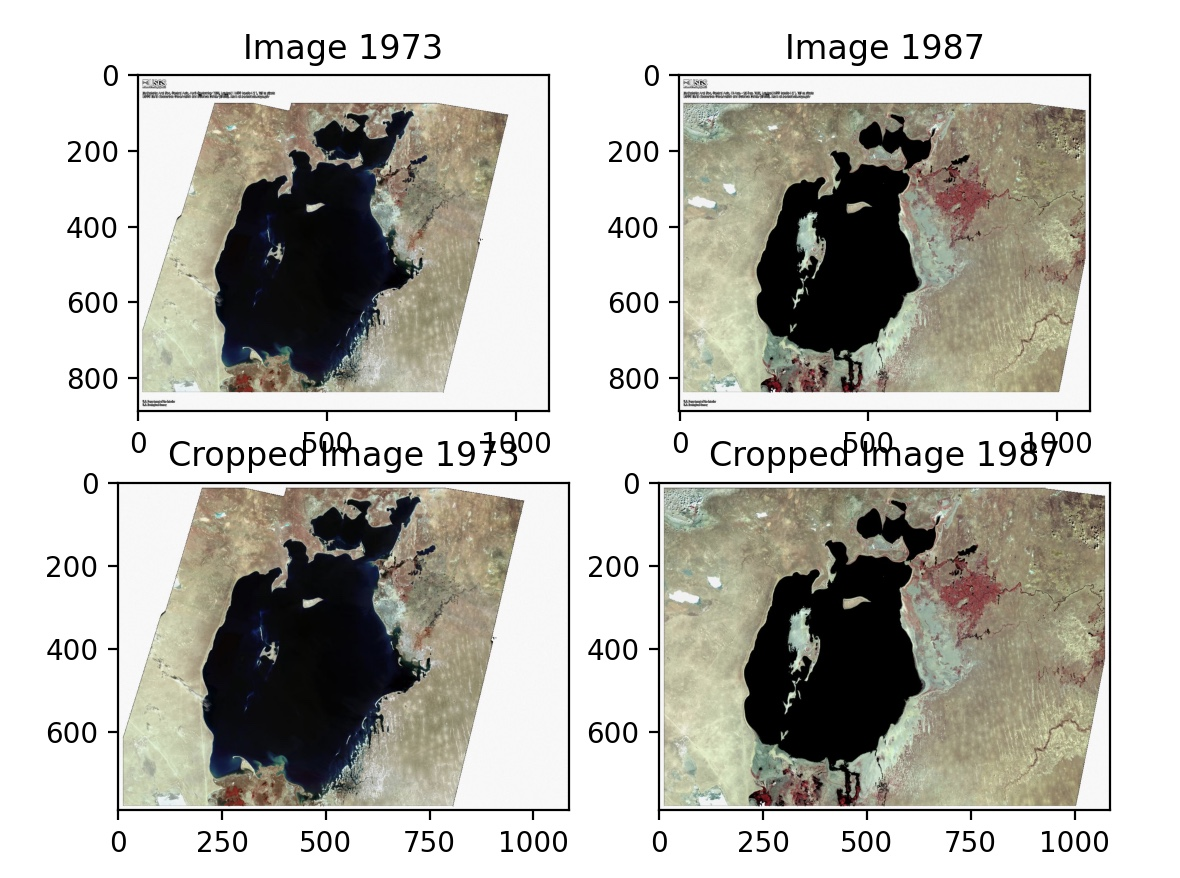
\includegraphics[width=0.65\textwidth]{./img/2.4.jpg}
            \caption{\label{fig:1.2}Images tronquées}  
        \end{center}
\end{figure}

\clearpage








